\section{Motivation for Message Aggregation}\label{sec:motivation_for_aggregation} 

In Chapel, a program's data access patterns and the programmer's choice of data distribution greatly influence the program's runtime and communication behavior. There are some situations where programs exhibit predictable patterns of communication that the compiler can detect. In doing so, the compiler can aggregate remote data elements coming from one locale into one local buffer via a single message and then access this local buffer on subsequent iterations of the loop. 

For example, consider Chapel code for the Jacobi computation shown in Figure \ref{jacobi_code}, a common stencil operation that computes elements of a two dimensional array as an average of that element's four adjacent neighbors. On each iteration of the loop, five array elements are accessed in an affine manner: the current array element $A_{new}[i, j]$ and its four adjacent neighbors $A[i+1, j]$, $A[i-1, j]$, $A[i, j+1]$, and $A[i, j-1]$. Naturally, the computation will take place on the locale of $A_{new}[i, j]$, the element being written to. If arrays $A$ and $A_{new}$ are distributed with a Cyclic distribution as shown in Figure \ref{cyc_dist}, then it is guaranteed that $A[i+1, j]$, $A[i-1, j]$, $A[i, j+1]$, and $A[i, j-1]$ will not reside on the same locale as $A_{new}[i, j]$ \textbf{for all iterations of the loop}. These remote elements are transferred over to $A_{new}[i, j]$'s locale in four individual messages during every loop iteration. For large data sets, transferring four elements individually per loop iteration drastically slows down the program because the message overhead is incurred more than once. 

Because the data is distributed using a Cyclic distribution, we notice that the data is accessed in the same way every cycle. Consider two iterations that are on different cycles, $(i, j) = (2, 2)$ and $(i, j) = (4, 2)$. Both iterations of the loop take place on locale 3, and both access 2 remote data elements from locale 1 and 2 remote data elements from locale 2. The remote data elements being accessed each cycle are a known fixed distance away from each other within the array $A$. We can therefore bring in all remote data elements accessed by iterations where $A_{new}[i, j]$ resides on locale 3 to locale 3 before the loop executes, access them from this local storage, and write them back to locales 1 and 2 after the loop finishes. Figure \ref{aggregation} illustrates this process in detail. 

If we focus on locale 3, there will be four buffers containing remote data elements after aggregation has occurred, one for each affine array access in the loop in Figure \ref{jacobi_code}. Now that a copy of all remote data elements reside on the locale that they are used from, the affine array accesses other than $A_{new}[i, j]$ can be replaced with accesses to the local buffers. After the loop has finished, any buffer elements that have been written to are communicated back to their respective remote locales in their own aggregate messages. This optimization can also be applied to the Block Cyclic distribution, as the data access pattern is the same for elements in the same position within a block. 

If arrays $A$ and $A_{new}$ are instead distributed using Chapel's Block or Block Cyclic distributions as shown in Figure \ref{block_dist} and Figure \ref{block_cyc_dist} respectively, the program will only perform remote data accesses on iterations of the loop where element $A_{new}[i, j]$ is on the boundary of a block. As the block size increases, the number of remote data accesses for the Jacobi computation decreases. For the Jacobi computation, it is clear that distributing the data using Chapel's Block distribution is the best choice in terms of communication. Executing the program using a Block distribution will result in fewer remote data accesses than when using a Block Cyclic distribution. Similarly, executing the program using a Block Cyclic distribution will result in fewer remote data accesses than when using a Cyclic distribution. 

It is important to note that the Block distribution is not the best choice for all programs using affine array accesses. Programs with strided access patterns that use a Block distribution will have poor communication performance because accessed array elements are more likely to reside outside of a block boundary. For these types of programs, a Cyclic or Block Cyclic distribution will perform better. 

\begin{figure}
\begin{center}
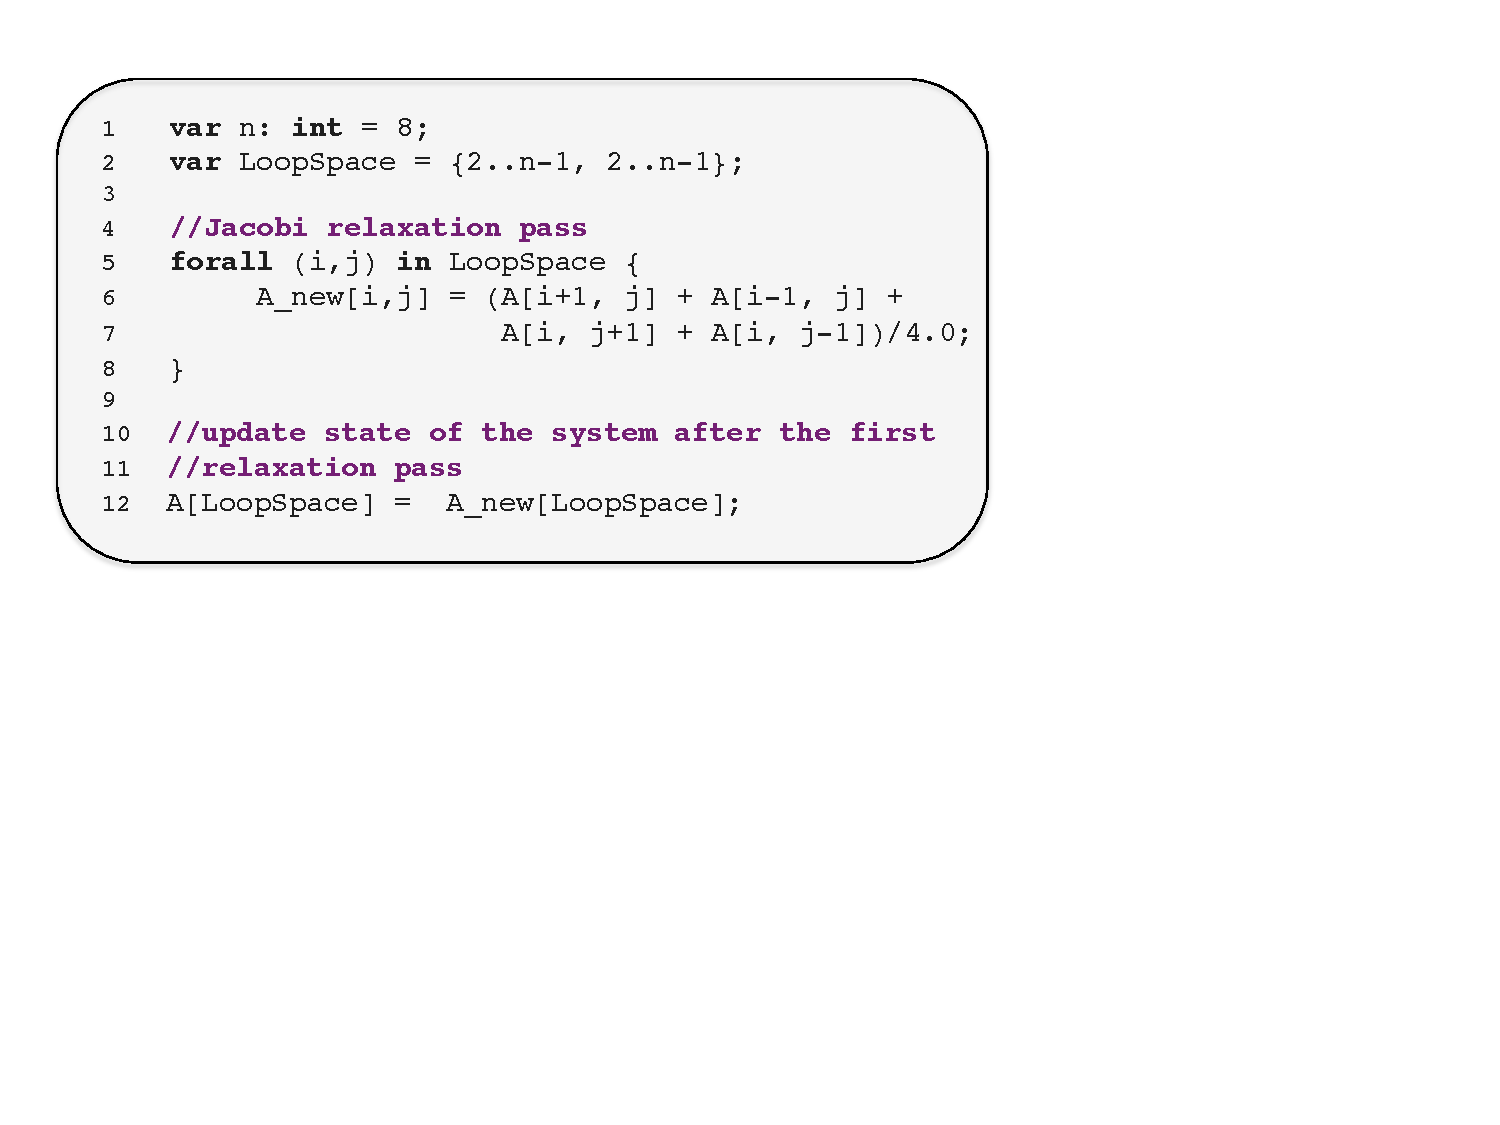
\includegraphics[scale=0.55]{./Figures/jacobi}
\caption{Chapel code for Jacobi computation over an 8 x 8 two dimensional array. Arrays $A$ and $A_{new}$ are distributed with a Cyclic distribution and their declarations are not shown. During each iteration of the loop, the current array element $A_{new}[i, j]$ gets the average of the four adjacent array elements of $A[i, j]$.}
\label{jacobi_code}
\end{center}
\end{figure}

\begin{figure}
\begin{center}
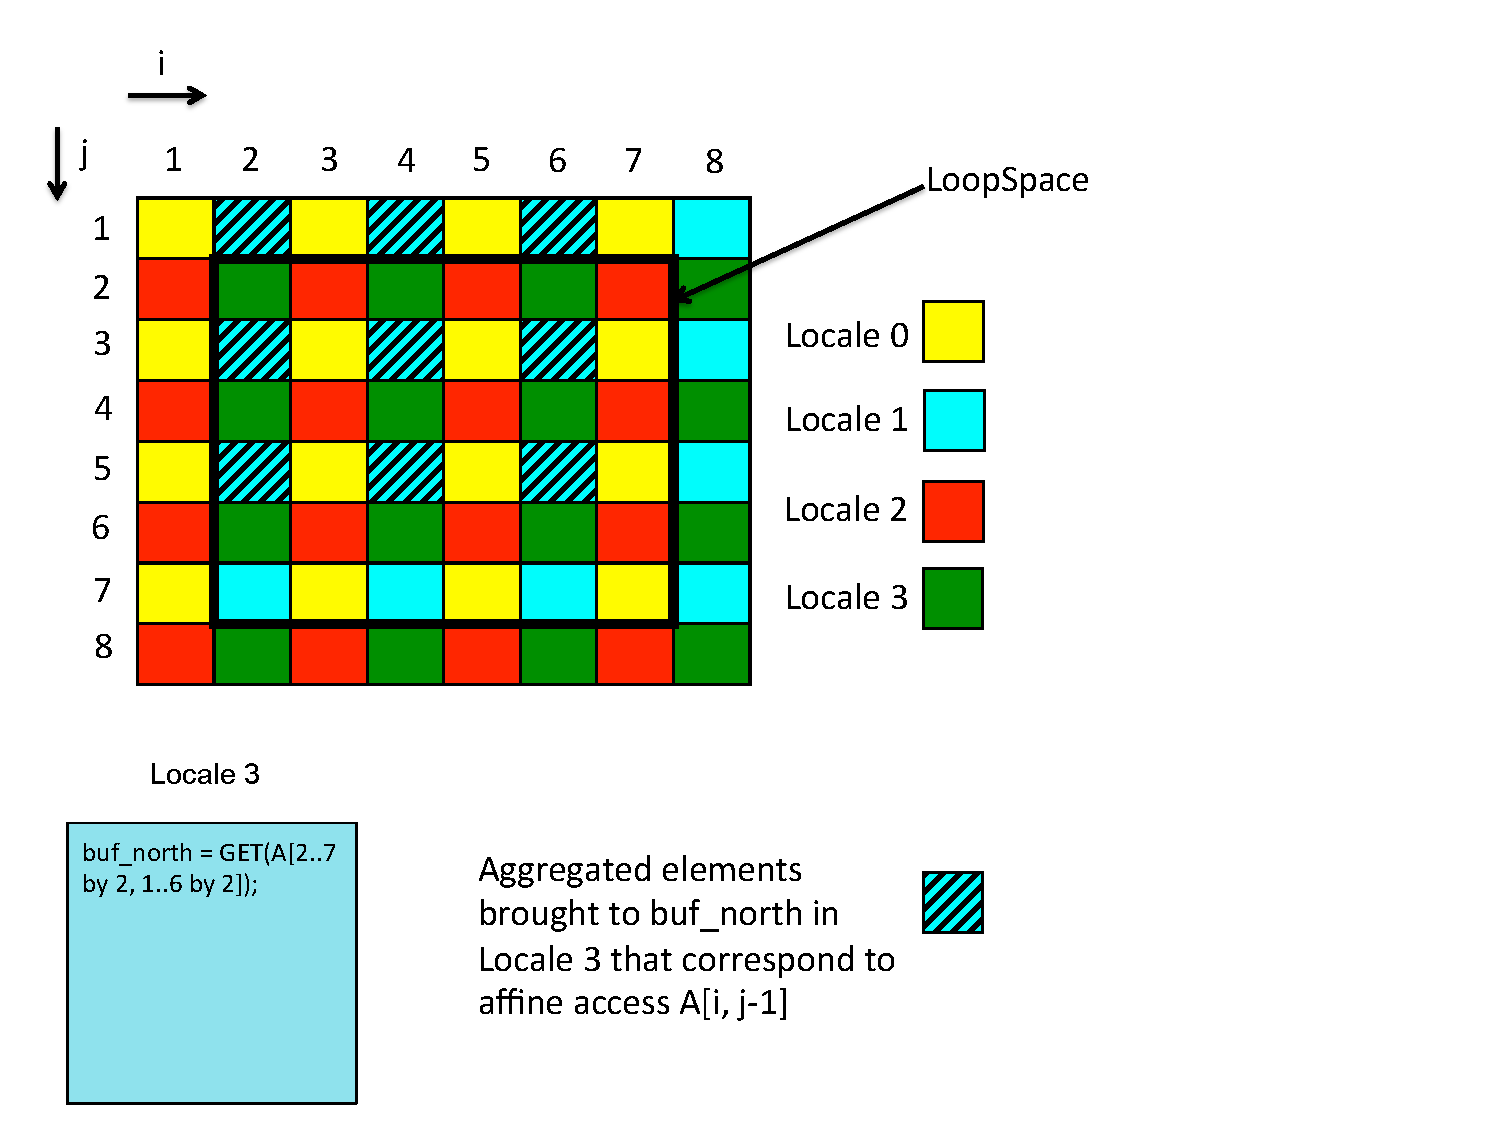
\includegraphics[scale=0.53]{./Figures/aggregation}
\caption{Illustration of message aggregation for the $A[i, j-1]$ affine array access of the Jacobi relaxation computation. The region \textit{LoopSpace} follows from Figure \ref{jacobi_code}. When $(i, j) = (2, 2)$, $A_{new}[2, 2]$ resides on locale 3. $A[2, 1]$ corresponds to the $A[i, j-1]$ access during this iteration, and it resides remotely on locale 1. If we now look at the next iteration where $A_{new}[i, j]$ resides on locale 3 (the next cycle, which is $(i, j) = (4, 2)$), we see that $A[4, 1]$ also resides on locale 1. We notice a pattern that all remote data accesses with respect to locale 3 corresponding to the $A[i, j-1]$ access in the loop \textbf{form an array slice $A[2..7$ $by$ $2, 1..6$ $by$ $2]$}, which we can aggregate with a single GET call and bring into $buf$\_$north$ on locale 3 before the loop begins. The array slice contains strided accesses of 2 in both the $i$ and $j$ dimensions, denoted using the Chapel keyword \textit{by} within the array slice. The striped elements form the elements that have been aggregated. This same procedure occurs on each locale for each affine array access that is deemed to be remote for all iterations of the loop.}
\label{aggregation}
\end{center}
\end{figure}


